\chapter{Monte Carlo Methods}
\graphicspath{{Chapter2/figures/}}
\label{ch:mcmethods}
This chapter reviews some fundamental concept in Monte Carlo method that are related to this thesis. It begins with a brief introduction to basic methods such as perfect Monte Carlo sampling, rejection sampling, importance sampling. It then details two common Markov Chain Monte Carlo (MCMC) techniques, namely Metropolis-Hastings and Gibbs Sampling. Lastly, it introduces the Sequential Monte Carlo (SMC) technique used in this thesis.

\section{Bayesian Inference}
In Bayesian inference framework, each unknown parameter in the model is assumed to be random variable and is  associated with prior distribution that characterises the initial belief. The inference process is merely updating the belief with new observable evidence in a systematic fashion using Bayes theorem.

Formally, let $M$ be the Bayes model of interest, $\theta$ be the set of parameters of the model, $p(\theta \mid M)$ be the prior distribution (initial belief) and $p(x \mid \theta, M)$ be the probability of observing an observation $x$ given the model, then posterior distribution (updated belief) is given as follows:  
\begin{align}
  p(\theta \mid x , M) &= \frac{p(x \mid \theta , M)~p(\theta \mid M)}{p(x \mid M)} \nonumber \\
                   &\propto p(x \mid \theta , M)~p(\theta \mid M) \label{eq:bayes} \\
  \text{posterior} &\propto \text{likelihood} \times \text{prior}
\end{align}

This problem formulation is elegant, but there remains some subtle issues in practice. One particular issue is about the calculation of the normalisation constant $p(x \mid M)$ in \eqref{eq:bayes}, which requires us to have the ability to carry out the following integral analytically:
\begin{equation}
  p(x \mid M) = \int p(x \mid \theta, M) p(\theta \mid M)~d\theta
\end{equation}
, which is often infeasible\footnote{Traditionally, the need of normalisation constant is often circumvented by making use of conjugate prior (the choices of certain prior distributions that yield posterior distributions from the same family) in an analytical fashion.}.

Instead of a closed form solution, the Method Carlo methods offer a numerical solution in estimating the integral using sampling technique. The need of calculating integral that does not posess analytic solution also arises in the marginalisation process of nuisance parameters, calculating expectation of a function, etc..

\section{Perfect Monte Carlo}
Consider the calculation the expectation of a function, $I$ of the following form:
\begin{equation}
  I = E[f(x)] = \int f(x)p(x)~dx
\label{eq:expectation}
\end{equation}
assuming we are able to sample $N$ independent and identically distributed (i.i.d.) points of $x$ from $p(\cdot)$, denote these as $\{x^{(i)}\}$ where $i$ is from $1 \ldots N$, a Monte Carlo estimate of $I$ using the the point masses of the samples is:
\begin{equation}
  \hat{I} = \frac{1}{N} \sum^N_{i=1} f(x^{(i)})
\end{equation}
One can view this approximation as a discretisation of the continuous distribution with \emph{random} support. This estimate has been shown to be unbiased and converge almost surely to be unbiased and converge almost surely to $I$ as $N \rightarrow \infty$ by the Law of Large number.

Morever, if the variance of $f(\cdot)$ is bounded ($\sigma^2_f < \infty$), then the following central limit theorem holds:
\begin{equation}
  \sqrt{N}(\hat{I} - I) \Longrightarrow N(0, \sigma^2_f)
\end{equation}
as $N \rightarrow \infty$, where $\Longrightarrow$ denotes convergence in distribution. It is important to note that the converengence rate of $\frac{1}{\sqrt{N}}$ is independent of the dimensions of $x$. This is in constrast with any determinstic method that has a rate that decreases a the integral dimension increases \cite{RCP05}. This is the main advantage of Monte Carlo integration.

\section{Rejection sampling}
However, it is not always possible to sample directly from the distribution $p(\cdot)$. Suppose we can find an instrumental distribution, $q(\cdot)$, that is easy to sample from and has the property such that $cq(x)$ dominates $p(x)$ for all $x$, i.e., $cq(x) \geq p(x) \geq 0$ for all $x$, then to get a random sample from $p(\cdot)$, we can first sample from $q(\cdot)$ instead and accept the sample with acceptance probability $\alpha(x)=\dfrac{p(x)}{cq(x)}$. If the sample is rejected, repeat the process until success. The algorithm is summarised in Algorithm \ref{algo:rejectionsampling}.

\begin{algorithm}
\caption{Rejection Sampling}\label{algo:rejectionsampling}
\begin{algorithmic}[1]
\Function{RejectionSampling}{n}
\State $r = [\ ]$
\Repeat
  \State sample $x \sim q(\cdot)$
  \State sample $u \sim {\cal U}(0,1)$
  \If {$u \leq \dfrac{p(x)}{cq(x)}$}
    \State $r \gets [r,x]$
  \EndIf
\Until{len(r)=n}
\EndFunction
\end{algorithmic}
\end{algorithm}

One could easily see that the optimal choice of instrumental distribution, $q^*$, is that one minimize the space bounded by $cq(x)$ subject to the constraint that it still dominates the target density $p(x)$. As the dimension of $x$ increases, this algorithm becomes very ineffecient because the acceptance ratio that is defined as the ratio of two embedded spaces tends towards zero and therefore many generated examples would be rejected. 

\section{Importance sampling}
\label{sec:IS}
Instead of making a binary accept-reject decision on each sample, the main idea behinds important sampling is to weight each sample $x$ based on how well the sample from the instrumental distribution, $q(\cdot)$, resembles the target distribution, $p(\cdot)$. More formally, assume we have an instrumental distribution, $q(\cdot)$, that is easy to sample from which has support that includes $p(\cdot)$, we can re-write \eqref{eq:expectation} as:
\begin{align}
  I &= \int f(x)\dfrac{p(x)}{q(x)}q(x)~dx \nonumber \\
    &= \int f(x)w(x)q(x)~dx
\end{align}
where $w(x)=\dfrac{p(x)}{q(x)}$, which is commonly referred as the importance weight. This reformulation leads to the following Monte Carlo estimate of $I$:
\begin{align}
  \hat{I} &= \dfrac{\frac{1}{N} \sum^N_{i=1} w(x^{(i)})f(x^{(i)})}{\frac{1}{N} \sum^N_{j=1} w(x^{(j)})} \nonumber \\ 
          &= \sum^N_{i=1} \tilde{w}(x^{(i)}) f(x^{(i)}) \label{eq:is}
\end{align}
where $\tilde{w}(x^{(i)})=\dfrac{w(x^{(i)})}{\sum^N_{j=1}w(x^{(j)})}$ is the normalised importance weight. This estimate is biased as it consists of the ratio of two estimates, yet it is still asymtoptically consistent.

To obtain samples from the target distribution, $p(\cdot)$, an additional resampling step can be introduced. In the first step, we sample a sample set of size $M$, ${\tilde{x}^{(i)}}_{0 \leq i \leq N}$ from the instrumental distribution, each of whcih is associated with a weight $\tilde{w}(x^{(i)})$ as discussed. In the resampling step, a sample set of $N$, ${\tilde{x}^{(i)}}_{0 \leq i \leq N}$ is draw from this intermediate set with the weightings taken into account. 

There are many ways of implementing the resampling stage. A simple direct implementation would be select the sample from the intermediate stage according to a Multinomial distribution with with the success probability parameter set to the weighting vector, $\tilde{w}(x^{(i)})_{0 \leq i \leq N}$, i.e., the chance of a sample point being replicated is proportional to its weightings. Note that this resampling step introduces extra variance to the estimators, but it is crucial in the sequential scheme that we shall look in the following section to avoid sampling degeneracy over time.

\section{Sequential Monte Carlo}
\label{sec:SMC}
Even if we were able to sample exactly from the target distribution $\pi_n(x_{1:n})$, the minimal computational complexity of the sampling scheme would be at least linear in $n$. Sequential Monte Carlo (SMC) techniques provides a way to obtain samples for each sequential time step in a fixed computational complexity time in Hidden Markov Models (HMMs). We shall briefly some background on HMMs in the next section that is necessary to understand SMC. Refer \cite{CO05} for further details of inference techniques for HMMs in general. 

\subsection{Hidden Markov Models}
HMMs can be seen as a class of models that consist of two related processes: an underlying Markov process, $X_t$, which is the target process of interest, and a observable process, $Y_t$, which its state can be measured and therefore provides some information about $X_t$. Moreover, it is assumed that these two processes have conditional independence properties as shown using the graphical model representation in Figure \ref{fig:HMM}. These properties can be summarised as follows:
\begin{align}
   p(x_t \mid x_{1:t-1}) &= f(x_t \mid x_{t-1})   \nonumber \\
   p(y_t \mid x_{1:t}, y_{1:t-1}) &= g(y_t \mid x_{t}) 
\end{align}
where $f(x_t \mid x_{t-1})$ is the transition density and $g(y_t \mid x_t)$ is the likelihood. 
\begin{figure}
\centering
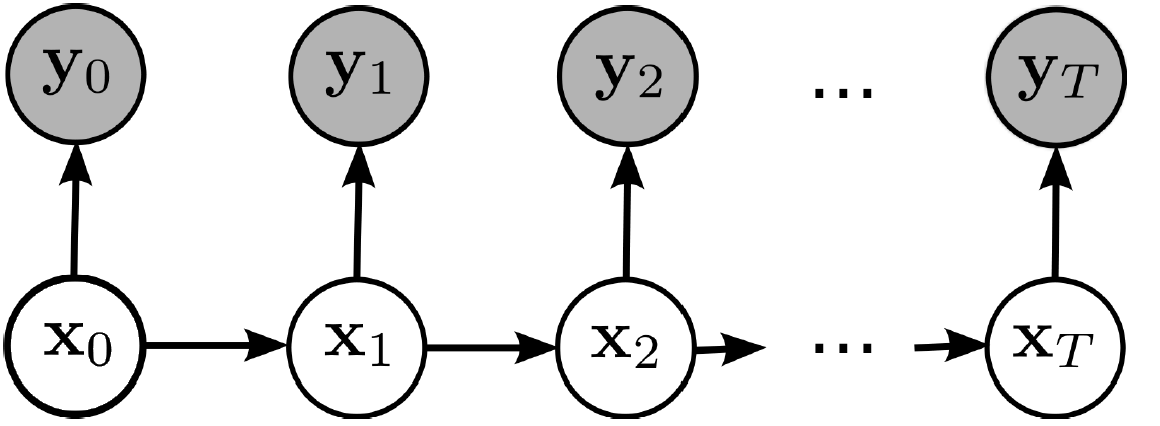
\includegraphics[width=0.7\textwidth]{hmm.png} 
\caption{Hidden Markov Models}
\label{fig:HMM}
\end{figure}
It is worth emphasizing here that this model is designed to capture systems that evolve from one state to another over time, generating observation after each state move. The inference problem is typically about estimating the state(s) in \emph{real-time} given the observations. This imposes an implicit requirement from the computation perspective that the estimate calculation cost should remain constant over time, i.e., the calculation cost does not increase with the increasing number of states.

Arguably, the most common inference problem in HMMs is the smoothing distribution, $p(x_{1:t} \mid y_{1:t})$, that is estimating the states $x_{1:t}$ based on the sequence of observations up to time $t$, $y_{1:t}$. Using Bayes rules, we can write the density of the distribution of interest as follows:
\begin{align}
    p(x_{1:t} \mid y_{1:t}) &\propto p(x_{1:t} \mid y_{1:t-1}) g(y_t \mid x_t) \nonumber \\
                            &= p(x_{1:t} \mid y_{1:t-1})f(x_t \mid x_{t-1})g(y_t \mid x_t)
\end{align}
This recursion is often re-written into two separate steps: the prediction step (the estimation of distribution of $t$ states given only $t-1$ states):
\begin{equation}
  p(x_{1:t} \mid y_{1:t-1}) = p(x_{1:t-1} \mid y_{1:t-1})f(x_t \mid x_{t-1}) \nonumber \\
\end{equation}
and the update step (the correction of the predicted distribution taking into account the new observation as follows:
\begin{equation}
  p(x_{1:t} \mid y_{1:t}) = \dfrac{p(x_{1:t} \mid y_{1:t-1}) g(y_t \mid x_t)}{\int p(x_{1:t} \mid y_{1:t-1}) g(y_t \mid x_t)~dx_{1:t}}
\end{equation}
Moreover, the estimate of any smoothing distribution $p(x_{j:k} \mid y_{1:t})$ where $j \leq k \leq l)$ can be obtained by integrating out $x$ that are not interested in as follows:
\begin{equation}
  p(x_{j:l} \mid y_{1:t}) = \int p(x_{1:t} \mid y_{1:t}) dx_{1:j, l+1:t}
\label{eq:smoothing}
\end{equation}
One particular smoothing distribution of interest is the final marginal distribution $p(x_t \mid y_{1:t})$, which is often referred to as the filtering distribution.

Another distribution of interest is  the prediction distribution, that is the estimation of the distribution of any unseen \emph{future} state based on the sequence of observations up to time. If we let $j = 1$ and $l \geq n$ in \eqref{eq:smoothing}, we obtain the following equation:
\begin{equation}
  p(x_{j:l} \mid y_{1:t}) = p(x_{j:t} \mid y_{1:t}) \prod^k_{i=t+1} f(x_i \mid x_{i-1})
\end{equation}
Therefore, any prediction density can be obtained by simply integrating out the variables of not interest from the above equation.

While the problem of distribution estimations as discussed appears to be simple, but the problem is in fact far from being resolved in practice. The integral appear in the above equations are often intractable and can only be estimated except in the a very specific setting discussed below.

\subsection{Kalman Filter}
In the linear Gaussian setting in which the transition density and likelihood are each a Gaussian distribution with center lied at a point of a linear combination of the known conditional variables, $u_t$ of the following form:
\begin{align}
  f_t(x_t \mid x_{t-1}, u_t) &= N(A_t(u_t) x_{t-1} + F_t(u_t), B_t(u_t)B_t(u_t)^T) \nonumber \\
  g_t(y_t \mid x_t, u_t)    &= N(C_t(u_t) x_t, D_t(u_t)D_t(u_t)^T)
\end{align}
where $A_t$, $B_t$, $C_t$, $D_t$ are appropriate known matrix or vector operations, that may depend on the given conditional variable $u_t$.

Using the properties of Gaussian distribution, the integral can be resolved analytically. This leads the widely used \emph{Kalman Filter} \cite{KRE60}, which has the following recursive solution as follows:
\begin{align}
  \mu_{t \mid t -1} &= A_{t}(u_t)(\mu_{t-1 \mid t-1})X_{t-1} + F_t(u_t) \\
  \Sigma_{t \mid t -1} &= A_{t}(u_t)\Sigma_{t -1 \mid t -1}A_{t}(u_t)^T +  B_t(u_t)B_t(u_t)^T \\
  S_t &=  C_{t}(u_t)\Sigma_{t \mid t -1}C_{t}(u_t)^T +  D_t(u_t)D_t(u_t)^T \\
  y_{t \mid t-1} &=  C_{t}(u_t)  \mu_{t \mid t -1} + G_t(u_t) \\
  \mu_{t \mid t} &=   \mu_{t \mid t -1} +   \Sigma_{t \mid t -1} C_{t}(u_t)S_t^{-1}(y_t - t_{t \mid t-1}) \\
  \Sigma_{t \mid t} &=  \Sigma_{t \mid t -1} -\Sigma_{t \mid t -1} C_{t}(u_t)S_t^{-1} C_{t}(u_t)\Sigma_{t \mid t -1}
\end{align}
where  $\mu_{t \mid t -1}$ and $\Sigma_{t \mid t -1}$ are the predicted mean and covariance of the state $x_t$, $y_{t \mid t-1}$ and $S_t$ are the mean and covariance of the measurement at time $t$ and $\mu_{t \mid t}$ and $\Sigma_{t \mid t}$ are the estimated mean and covariance of the state $x_t$ after seeing the observation $y_t$.

There are various extensions have been developed to this approach. For example, the Extended Kalman Filter (EKF) which uses Taylor Series expansion to linearise at the conditional variables locally, Unscentend Kalman Filter, etc. Refer \cite{WG95} for further details.

\subsection{Sequential Important Sampling (SIS)}
In more general setting, here is however no analytical solution for this estimation problem. Sequential Monte Carlo provides a systematic way to approximate the solution to this estimation problem. Assuming that it is possible to decompose the selected importance distribution in the following form:
\begin{align}
	q_n(x_{1:t}) &= q_n(x_{1:t-1}) q_n(x_t \mid x_{1:t-1}) \nonumber \\
	             &= q_1(x_1) \prod^n_{i=2} q_i(x_i \mid x_{1:t-1})
\end{align}
we can then obtain sample of ${X_{1:n}} \sim q_n(x_{1:t-1})$ at time $t$ by first sample $X_1 \sim q_1$ at time $1$ then $X_i \sim q_i(x_i \mid x_{1:t-1})$ for time $i$ from $2 \ldots n$. The corresonding weights associated to each sample $X_{1:n}$ can also calculated in a similar recursion fashion using the following decomposition:
\begin{align}
  w_n(x_{1:t}) &= \frac{p_t(x_{1:t})}{q_t(x_{1:t})} \nonumber \\
               &= \frac{p_{t-1}(x_{1:t-1})}{q_{t-1}(x_{1:t-1})} \frac{p_t(x_{1:t})}{p_{t-1}(x_{1:t-1})q_n(x_t \mid x_{1:t-1})} \label{eq:w} \\
  &= w_1(x_1) \prod^n_{i=2} \frac{p_i(x_{1:i})}{p_{i-1}(x_{1:i-1})q+n(x_i \mid x_{1:i-1})} \nonumber \\
  &= w_1(x_1) \prod^n_{i=2} \alpha_k(x_{1:i})
\end{align}
where $\alpha_k(x_{1:i})$  is often referred to as incremental importance weight function. This algorithm is summarised in X.

\subsection{Optimal Proposal Distribution}
While SIS is attractive, it is nothing but a specialised version of importance sampling introduced earlier in \ref{sec:IS}. As the state space increases with the number of time step $t$. Direct importance sampling on a state space with increasing size is not efficient. The weights of the samples start to degenerate quickly, in the sense that the weights start to concentrate on only a small number of samples, i.e., many of the samples have negligible weights and therefore rendered useless in estimating the expectation. It can be shown that the importance weights will increase with every iteration, and therefore the quality of the estimators will decrease over time \cite{}. 

To alleviate this weight degeneracy issue, we can rewrite \eqref{eq:w} as follows:
\begin{align}
 w_n(x_{1:t}) &= \frac{p_{t-1}(x_{1:t-1})}{q_{t-1}(x_{1:t-1})} \frac{p_t(x_{1:t})}{p_{t-1}(x_{1:t-1})q+n(x_t \mid x_{1:t-1})} \nonumber \\
              &= 1+1
\label{eq:w2}
\end{align}
Looking at \eqref{eq:w2}, it is obvious that the proposal distribution, $q_{t+1}$ that minimise the variance of the importance weight, $w_n(x_{1:t})$ takes the following form:
\begin{equation}
 q_{t+1}(x+1 \mid x_{t-1} \propto f_{t+1}(x_{t+1} \mid
\end{equation}
This is often referred to as the optimal proposal distribution.

In general, it is not always possible to sample from this optimal proposal distribution. Yet, the knowledge of its form can be used to guide the design of a reasonable good proposal distribution, which can be sampled from. Using a better proposal distribution reduces the amount of variance introduced, but does not totally eliminate degeneracy problem.

\subsection{Sequential Importance Resampling (SIR)}
The variance in importance weight accumulates over iterations. This suggests a possible solution is to ``reset'' the weights associated to the samples somehow during the iterations. Sequential Importance Resampling (SIR) introduces an additional resampling step to SIS step in a similar fashsion as discussed in Section \ref{sec:IS}. After resampling, the weight of each samples are reset to be equal, i.e., $\frac{1}{N}$. This algorithm is summarised in X.

Besides the simpliest multinomial resampling scheme, many different resampling schemes have been proposed in the literature. For example, stratified resampling \cite{} as the name suggested splitting the samples in stratums to ensure the good coverage on the resulting sample set, residual resampling \cite{} that has an effect in reducing the variance of the weights, etc. See \cite{} for further details on the comparison of these sampling schemes.

However, resampling is not a silver bullet for sampling imporishment. Essentially, resampling provides a mechanism to eliminate low weight samples to give way to replicate \emph{copies} of high weight samples. This allows all samples to participate and contribute to forma  good estimation of the distribution of interest. This is obvious for the case of estimating filtering distribution and predictive distribution.

Over time, this replication reduces the number of distinct values available for previous time steps. The start of the trajectory will eventually become the same. This phenomena is known as sample impoverishment. This is a fundamental weakness of SMC, in which the history of the path is not re-written. The lose of diversity in the sample set will have a negative impact when it comes to estimating snoothing distribution.

\subsubsection{Resample-Move Algorithm}
To counteract this sample impoverishment, Resample-Move Algorithm \cite{} is proposed to introduce some perturbance to the samples (so to diversify them) without changing the distribution they represent. This is accomplished by using MCMC steps with a Markov Kernel, $K$ that is invariant to the target distribution.

In the original paper, this is done in a way by introducing an additional MCMC ``move'' step to each sample after resampling step according to a Markov kernel that is invariant to the target distribution. This algorithm is summarised in X.

This does not entirely solve the smoothing distribution estimation problem. To apply Markov Kernels with invariant distribution corresponding to the smoothing distribution, the space that Markov kernel is defined has to increase at each iteration. This implies the computation time increases linearly with time. Moreover, fast mixing high dimension Markov kernel in itself is not easy to design. In practice, one could use a sliding windows approach, in which MCMC Kernels which diversify the samples of the previous $n$ time step at each iteration. This has a \emph{fixed} additional cost to each iteration.

\subsection{Effective sample size (ESS)}
Resampling step induces additional Monte Carlo variance to the weights. Yet, this step is necessary to avoids accumulation of estimation variance on weights over time and therefore result in a more stable approximation to the filtering and preditive distribution.

To trading off these two competing requirements, one possible way to monitor the effective sample size (ESS) which provides a measure on the quality of the weighted samples. Two possible estimation are as follows:
\begin{equation}
  ESS \approx \dfrac{1}{E[w^2]} \approx \dfrac{\left(\sum^N_{i=0} w_i \right)^2}{\sum^N_{i=0}w_i^2}
\end{equation}
A possible implementation is that resampling step is only triggered if the $ESS_t$ faill below certain threshold at time $t$, say $N/2$. See \cite{} for detail discussion on ESS.

\subsection{Rao-blackwellised (Marginal) Important sampling}

\section{Conclusion}
This chapter presents a review of Monte Carlo method, with a particular focus on Sequential Monte Carlo method that is used extensively in this thesis for portfolio optimisation. It begins to describe traditional Monte Carlo sampling techniques. It then introduce a simple SMC algorithm, and couple of extensions that have been proposed to improve the performance of the algorithm. Lastly, the chapter presents a simple concrete example, in which SMC is used to estimate the filtering and smoothing distribution for the problem in question.

It is worth nothing the algorithm is not restricted to sequential filtering problem. For example, it has been established that it is possible to use SMC within MCMC framework (pMCMC, where p stands for particle) \cite{pMCMC} to solve other problems. In the next chapter, we will show Sequential Monte Carlo is used as a maximiser to search for a optimal strategy for a portfolio, given a multiplicative reward function.

\endinput
\section{Markov chain Monte Carlo (MCMC)}
%The rejection and importance algorithms scale badly with dimensionality. In some problems, it may still possible to decompose the probability distribution of interest, $P(x_{1:N})$ into low dimensional conditional distributions and proceed from there. However, this is not often feasible in practice.

Markov chain Monte Carlo (MCMC) are a set of algorithms that allows ones to draw random samples from the target probability distribution by constructing a ergotic Markov chain process which has its stationary distribution set to be target desired distribution. 

\subsection{Markov Chain}
Conceptually, Markov chain is a stochastic process in which the past and future states of the process are independent given the current state. A Markov chain can be viewed as an \emph{ordered} sequence of states $\{x_{1:N}\}$, in which state $x_t$ only depends on state $x_{t-1}$, i.e., the state at time $t$ is determined based on some trasition distribution of the form $p(x_t \mid x_{t-1})$, which is independent of all previous states $x_{t-2}, x_{t-3}, \ldots$. 

To ensure the Markov chain converges to a steady state (stationary distribution), the chain needs to satisfy the following properties:
\begin{enumerate}
\item irreducible --- no matter where it starts a chain, it is possible to reach all other states in finite amount time steps.
\item aperiodic --- 	for all the states $i$, the chain can  return to state $i$ at irregular time.
\item positive recurrent --- for all the state $i$, the chain will definitely revisit the state in finite amount time stpes.
\end{enumerate}

In practice, it is usually not difficult to construct the required Markov Chain, the more difficult problem is to determine how many steps it takes to converge, often known as mixing. Various visual diagnostic have been developed, yet it is often a matter of art. Refer \cite{RCP05} for details.

In the following sections, we present two basic MCMC algorithms: Metropolis Hastings algorithms, Gibbs algorithms and a third algorithm in which these two basic algorithms are ``mixed and matched'' in a hierarchical fashion to form a more advanced samplers to fit application needs.

\subsection{Metropolis-Hastings sampling}
The first major MCMC algorithm was devised by Metropolis in \cite{MN53}. The algorithm constructs a Markov Chain by proposing a random walk step based a proposal distribution is symmetric, i.e., the probability of moving from state $t$ to state $t-1$ is the same as the probability of moving from state $t-1$ to state $t$ ($q(x_{t} \mid x_{t-1}) = q(x_{t-1} \mid x_{t}$). The proposed step is then either accepted or rejected according to an acceptance probability, $\alpha(x)= \min\left(1, \dfrac{p(x_t)}{p(x_{t-1})}\right)$, where $p(x)$ is the target probability density evaluated at $x$.

This algorithm was generalised by Hastings \cite{WKH70} to allow the use of non-symmetric proposal density, with an adjustment to the accenptance probability $\alpha(x) = \min\left(1, \dfrac{p(x_t)q(x_t \mid x_{t-1})}{p(x_{t-1})q(x_{t-1} \mid x_{t})}\right)$ and hence the name, Metropolis-Hastings sampling. This algorithm is summarised in Algorithm \ref{algo:metropolishastings}.

\begin{algorithm}
\caption{MetropolisHastings}\label{algo:metropolishastings}
\begin{algorithmic}[1]
\Function{MetropolisHastings}{n}
\State $r = [\ ]$
\Repeat
  \State sample $x_t \sim q(x_{t-1})$
  \State sample $u \sim {\cal U}(0,1)$
  \If {$u \leq \min\left(1, \dfrac{p(x_t)q(x_t \mid x_{t-1})}{p(x_{t-1})q(x_{t-1} \mid x_{t})}\right)$}
    \State $x_{t-1} \gets x_{t}$
    \State $r \gets [r,x_{t-1}]$
  \EndIf
\Until{len(r)=n}
\EndFunction
\end{algorithmic}
\end{algorithm}

It is not hard to see that the algorithm works best if the density $q$ matches the shape as density $p$, which is often unknown. Assuming a Gaussian proposal density $q$ is used, there is also an addtional parameter, namely the variance $\sigma^2$ is required to be tuned. There is a trade-off to be made in the tuning process. If the $\sigma^2$ is set too be too small, the chain is likely to mix slowly (i.e., the proposed step is likely to be accepted yet each successive move is very slow and therefore the chain will converge to target distribution $p$ at a slow rate). On the other hand, if $\sigma^2$ is too large, the proposed step is likely to be rejected as it is likely to hand in a region of much lower probability density and the chain will converge slowly again. Again, refer \cite{RCP05} for details on convergence dianogstic.

\subsection{Gibbs sampling}
Gibbs sampling \cite{GS84} is a special form of the Metropolis–Hastings sampling. The key idea in Gibbs sampling is to re-write the target multivariate distribution of interest as a product of conditional probability distributions of lesser number of parameters. A Markov Chain is then constructed to generate samples for each parameter \emph{in turn} from the conditional distributions with an acceptance rate $\alpha(x)=1$, i.e., accept all the samples.

More formally, suppose we would like to have obtain $k$ samples of $\mathbf{x}=(x_1,x_2,\ldots, x_n)$ from $p(x_1, \ldots, x_n)$, assuming we start with an initial value $\mathbf{x}^{0}$. For each sample $(\mathbf{x}^{i}: i \in \{1 \dots n\})$, sample $x_j^{(i)}$ from the conditional distribution $p(x_j|x_1^{(i)},\dots,x_{j-1}^{(i)},x_{j+1}^{(i-1)},\dots,x_n^{(i-1)})$. In other words, sample each variable from the distribution of that variable conditioned on all other variables, making use of the most recent values and updating the variable with its new value as soon as it has been sampled. The algorithm is summarised in Algorithm \ref{algo:gibbs}.

\begin{algorithm}
\caption{Gibbs}\label{algo:gibbs}
\begin{algorithmic}[1]
\Function{Gibbs}{n}
\State $r = [\ ]$
\State sample $x^{(0)}$
\Repeat
  \State sample $x^{(t)} \sim p(x_j|x_1^{(i)},\dots,x_{j-1}^{(i)},x_{j+1}^{(i-1)},\dots,x_n^{(i-1)})$
  \State $r \gets [r,^{t}]$
\Until{len(r)=k}	
\EndFunction
\end{algorithmic}
\end{algorithm}

There are variations of Gibbs sampling techniques. For examples, a blocked Gibbs sampling groups more than one variables and sample from the joint distribution conditioning on other variables. Refer \cite{RCP05} for details. 


% ------------------------------------------------------------------------


%%% Local Variables: 
%%% mode: latex
%%% TeX-master: "../thesis"
%%% End: 
